\documentclass[a4paper,11pt]{article}
\usepackage[margin=22mm]{geometry}
\usepackage{fontspec,amsmath,booktabs,graphicx,hyperref}
\setmainfont{STIXGeneral}
\setlength{\emergencystretch}{2em}
\begin{document}
\begin{center}{\Large Topic C: proofs and their costs}\\[4pt]Human Compression project\end{center}
The common paper, \emph{Changes of chamber generators and binary translation
groups}, supports four complete applications: Janko geometries (C1), halving
generalized cubes (C2), Petrials (C3), and equal-parameter polyhedra (C4).
The fixed comparison preserves forty source clauses, including their explicit
corrections, retained theorems and two excluded auxiliary assertions.

\paragraph{The complete written comparison.}
The common paper costs 27,131 characters and the four applications cost
44,146. The three available source PDFs contribute 60,256. If $x$ is the
unknown cost of the original L108 PDF, then
\[R_C^{\mathrm{written}}=\frac{x+60\,256}{71\,277}.\]
There is no numerical overall factor. The full 10,071-character Petrial
application remains in the denominator. Its source browser rendering fixes
the mathematical statement boundary, but is not a substitute PDF measurement.

Both complete GAP programs are required for the Janko application. Their
printed appendix costs 8,799, charged once, giving the separate comparison
\[R_C^{\mathrm{programs}}=\frac{x+60\,256}{80\,076}.\]
Counting the two full raw files instead gives denominator 79,600. This is an
alternative representation of the same programs, not an additional charge.

\begin{center}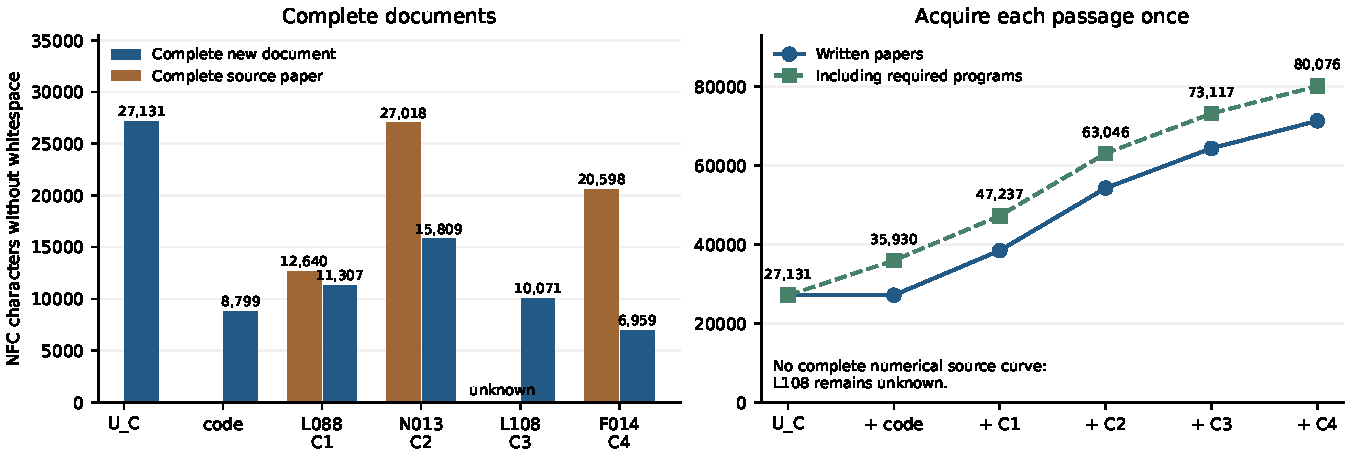
\includegraphics[width=\linewidth]{acquisition.pdf}\end{center}
\noindent All figures on this page use NFC characters without whitespace in
complete extracted PDF text, with the reviewed furniture exclusions and glyph
calibration. The same accounting is supplied for all thirty policy coordinates.
Unextracted graphics and expanded outside-proof costs remain unknown.

\paragraph{After acquiring the whole common theory and both programs.}
These are the admitted complete-source / complete-application factors.
\begin{center}\begin{tabular}{lrrr}\toprule
Source / application & Source & Application & Conditional factor\\\midrule
L088 / C1 & 12,640 & 11,307 & 1.118\\
N013 / C2 & 27,018 & 15,809 & 1.709\\
L108 / C3 & unknown & 10,071 & unknown\\
F014 / C4 & 20,598 & 6,959 & 2.960\\
\bottomrule\end{tabular}\end{center}
\newpage
\paragraph{A declared acquisition order.}
Acquire the complete $U_C$, the complete program appendix, and then C1,
C2, C3 and C4. Every application includes its definitions, title, context,
references and all proof passages. Let $K_i$ be the union of passage owners
paid by stage $i$. The new cost is $c(K_i\setminus K_{i-1})$; a prerequisite
already in $K_{i-1}$ is not charged again. No cost is shared across topics.
\begin{center}\begin{tabular}{lrrrr}\toprule
Added & New cost & Written total & With programs & Prior text used\\\midrule
U\_C & 27,131 & 27,131 & 27,131 & ---\\
CODE & 8,799 & 27,131 & 35,930 & ---\\
C1 & 11,307 & 38,438 & 47,237 & 17,032\\
C2 & 15,809 & 54,247 & 63,046 & 16,913\\
C3 & 10,071 & 64,318 & 73,117 & 5,161\\
C4 & 6,959 & 71,277 & 80,076 & 22,407\\
\bottomrule\end{tabular}\end{center}
The last column measures already acquired passages used by the complete local
paper's recorded arguments. It is not an extra subtraction from that paper's
cost. The historical cumulative written costs are 12,640, then 39,658,
then $x+39\,658$, and finally $x+60\,256$. Thus no complete numerical
historical acquisition curve is available. The sequence is a reading order,
not an estimate of research effort or a shortest possible proof.

\paragraph{What a smaller proof route measures.}
The paired graph records prerequisite-to-use arrows for each of the forty
clauses and for the four complete contracts. The additional identification of
the equal-parameter construction with the earlier polygon construction stays
separate. Each route's known cost is the union of its exclusive passage owners.
It can omit context still paid in the complete paper. Accordingly these route
subtotals are explanations, not replacement denominators or new compression
factors. Parent results and their proof branches may share a statement owner;
box costs overlap, while every total counts that passage once.

There are 156 graph nodes: 64 historical, 62 current, 26 retained external
inputs and four verification components, with 249 typed edges. Their categories
include definitions, statements and proof branches, at different levels of
detail. No node-count ratio is defined. The accounting has 199 text owners
and 195 selected-text spans. It also assigns excluded furniture to explicit
owners for the untrimmed sensitivity; no printed text is silently dropped.

\paragraph{Scope and verification.}
The accepted logical revision restores the seed and subgroup assumptions of
the historical Janko calculation without extending the string-only recognition
theorem to nonstring exercise cases. It records the historical halving C-group
premise and Cayley--Hamilton use, and keeps the current displacement proof
independent of unnecessary binary-module assumptions. Geometry is established
before naming the Janko residues. All source qualifications remain attached
to their original clauses.

The original L108 PDF, outside-proof expansions and graphic costs remain
unknown. The existing sixteen Lean declarations verify specified displacement,
intersection and semidirect-product components; they are not full formalizations
of the applications. The two complete Janko programs are preserved unchanged.
The cost checker verifies full-document conservation, unions and deliberate
corruptions. The offline HTML shows all proof routes, locations and unknown
inputs; its deterministic DOM test is not a real-browser layout test.
This new ownership and reader layer awaits independent review. It changes
no mathematical contract, source or question credit, or admitted paper factor.
\end{document}
